%%%%%%%%%%%%%%%%%%%%%%%%%%%%%%%%%%%%%%%%%
% Beamer Presentation
% LaTeX Template
% Version 1.0 (10/11/12)
%
% This template has been downloaded from:
% http://www.LaTeXTemplates.com
%
% License:
% CC BY-NC-SA 3.0 (http://creativecommons.org/licenses/by-nc-sa/3.0/)
%
%%%%%%%%%%%%%%%%%%%%%%%%%%%%%%%%%%%%%%%%%

%----------------------------------------------------------------------------------------
%	PACKAGES AND THEMES
%----------------------------------------------------------------------------------------

\documentclass{beamer}

\mode<presentation>
{

% The Beamer class comes with a number of default slide themes
% which change the colors and layouts of slides. Below this is a list
% of all the themes, uncomment each in turn to see what they look like.

%\usetheme{default}
%\usetheme{AnnArbor}
%\usetheme{Antibes}
%\usetheme{Bergen}
%\usetheme{Berkeley}
%\usetheme{Berlin}
%\usetheme{Boadilla}
%\usetheme{CambridgeUS}
%\usetheme{Copenhagen}
%\usetheme{Darmstadt}
%\usetheme{Dresden}
%\usetheme{Frankfurt}
%\usetheme{Goettingen}
%\usetheme{Hannover}
%\usetheme{Ilmenau}
%\usetheme{JuanLesPins}
%\usetheme{Luebeck}
	%\usetheme{Madrid}
	%\usetheme{Malmoe}
	%\usetheme{Marburg}
	\usetheme{Montpellier}
	%\usetheme{PaloAlto}
	%\usetheme{Pittsburgh}
	%\usetheme{Rochester}
	%\usetheme{Singapore}
	%\usetheme{Szeged}
	%\usetheme{Warsaw}

	% As well as themes, the Beamer class has a number of color themes
	% for any slide theme. Uncomment each of these in turn to see how it
	% changes the colors of your current slide theme.

	%\usecolortheme{albatross}
	%\usecolortheme{beaver}
	%\usecolortheme{beetle}
	%\usecolortheme{crane}
	%\usecolortheme{dolphin}
	%\usecolortheme{dove}
	%\usecolortheme{fly}
	%\usecolortheme{lily}
	%\usecolortheme{orchid}
	%\usecolortheme{rose}
	%\usecolortheme{seagull}
	%\usecolortheme{seahorse}
	%\usecolortheme{whale}
	%\usecolortheme{wolverine}

	%\setbeamertemplate{footline} % To remove the footer line in all slides uncomment this line
	%\setbeamertemplate{footline}[page number] % To replace the footer line in all slides with a simple slide count uncomment this line

	%\setbeamertemplate{navigation symbols}{} % To remove the navigation symbols from the bottom of all slides uncomment this line
}

\usepackage{graphicx} % Allows including images
\usepackage{booktabs} % Allows the use of \toprule, \midrule and \bottomrule in tables

%----------------------------------------------------------------------------------------
%	TITLE PAGE
%----------------------------------------------------------------------------------------

\title[Medical Image Registration]{A Survey of Medical Image Registration}
 % The short title appears at the bottom of every slide, the full title is only on the title page

\author{} % Your name
\institute[IIIT Vadodara] % Your institution as it will appear on the bottom of every %slide, may be shorthand to save space
{
	\section{\vspace{-10ex}}
	%\begin{flushleft}
	\medskip
	\textbf{Presented By -} \\ % Your institution for the title page
	
	
	\text{Vijay Deshpande (201761003)}
	

 % Your email address
}
 % Date, can be changed to a custom date

\begin{document}

\begin{frame}
\titlepage % Print the title page as the first slide
\end{frame}

\begin{frame}
\frametitle{Table of contents} 
\tableofcontents
\section{1.Introduction} 
\section{2.Classification}
\section{3.Trends}
\section{4.Challenges}
\section{5.Conclusion}
\end{frame}


\begin{frame}
\frametitle{Introduction}
\begin{itemize}
	\item The process of overlaying two or more images of the same scene with respect to a particular reference image.\\
	\item Images may be taken at various circumstances
	(time-points) and various perspectives (Viewpoints) .\\
	
\end{itemize}

\end{frame}

%%%%%%%%%%%%%%%%%%%%%%%%%%%%%%%%%%%%
\begin{frame}
\frametitle{Classification}
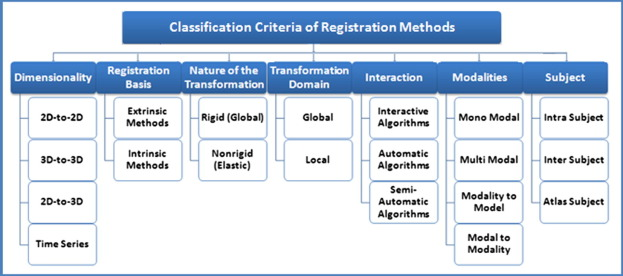
\includegraphics[width=11cm, height=7cm]{classi.png}
\end{frame}

%%%%%%%%%%%%%%%%%%%%%%%%%%%%%%%%%%%%
\begin{frame}
\frametitle{Nature of Registration}
\begin{itemize}
	\item \textbf{Rigid} : Described using a single constant matrix (a) \\ equation: $y_{i} = a_{ij}x_{j}$
	where x and y are the old and new coordinate vectors.
	\\
	\item \textbf{Non - Rigid} : Curved transformations cannot be represented using constant matrices .
 
	
	
\end{itemize}
\end{frame}

%%%%%%%%%%%%%%%%%%%%%%%%%%%%%%%%%%%%%
\begin{frame}
\frametitle{Domain of Registration}
\begin{itemize}
\item \textbf{Global} : Transformation is applied to entire image .
\item \textbf{Local} : Subsections of the image have their own transformations defined .
\end{itemize}
\end{frame}

%%%%%%%%%%%%%%%%%%%%%%%%%%%%%%%%%%%%
\begin{frame}
\frametitle{Recent Trends}
\begin{itemize}
	\item Shift from Extrinsic to Intrinsic Registration.
	
	\item No need to segment objects which are to be aligned.
	
	\item Consider the entire image as input.
	
	\item Several datasets with expert landmark annotations have become available.
	
	\item Few datasets have been setup for evaluation of registration methods.
	
	\item Annotated datasets are provided by DIRLAB, POPI, EMPIRE10, LONI, ADNI.
	
	\item EMPIRE10 was launched as evaluation challenge in conjunction with MICCAI 2010.
	
	

\end{itemize}


\end{frame}

%%%%%%%%%%%%%%%%%%%%%%%%%%%%%%%%%%%%
\begin{frame}
\frametitle{Challenges}

\begin{itemize}


\item Non-linear registration methods have not reached the status of inclusion in commercial software for lack of genericity and robustness.
\item Global rigid registration is currently the most frequently used registration in clinical approach.
\item Level of accuracy needed for clinical purpose is not known.
\item EMPIRE10 challenge is employed for registration evaluation.
\item Many mono-modal registration problems have been solved.
\end{itemize}





\end{frame}


%%%%%%%%%%%%%%%%%%%%%%%%%%%%%%%%%%%%%
\begin{frame}
\frametitle{Conclusion}
\begin{itemize}

\item There is a shift from extrinsic to intrinsic registration.
\item Shift from surface based registration to intensity based registration.
\item Emerging need of public database.
\item It has proven difficult to devise registration methods that are robust against the many variations encountered in clinical practice.e.g scanner type, scanning protocol, patient -characteristics.
\item Most mono-modality registration problems have been solved.


\end{itemize}
\end{frame}





\begin{frame}
\frametitle{References}
\bibliographystyle{ieeetr}
\bibliography{tech_writing}
\end{frame}

%------------------------------------------------

\begin{frame}
\Huge{\centerline{The End}}
\end{frame}

%----------------------------------------------------------------------------------------

\end{document} 